% Provenance (never printed): see sources/outline_sources.md (Year 2: sedimentary basins;
% subsidence curves and backstripping; the stretching model). Stretching model after McKenzie
% (1978) as restated by Sheplev and Reverdatto (1998) and coded in pyBacktrack (EarthByte);
% backstripping after pyBacktrack's well module; North Sea after Sclater and Christie (1980);
% Michigan after Sloss (1982) and Crowe et al. (2009); the US Atlantic margin after Schlee et
% al. (1976), Poag (1979) and Lang et al. (2024); the Molasse after the chapter 13 rows.
% Curves and the invented well from figdata/bachelor-2/basins.py; exercise and problem values
% in the Book 4 scratch calculator calc/ch16.py.
\chapter{Bassins sédimentaires comparés}\label{ch:b2:basins-compared}

Au large de la côte est des États-Unis, sous le plateau continental, le Baltimore
Canyon Trough contient au moins \qty{14}{km} de roches sédimentaires. Un forage qui traverse une telle
pile lit son histoire à rebours : chaque unité qu'il recoupe fut jadis le fond de la mer, à une
profondeur que les fossiles et les sédiments enregistrent, puis elle a été enfouie et comprimée.
La profondeur de chaque surface datée est un point d'une courbe d'enfoncement. Pourtant, la plus
grande part de l'enfoncement tient au poids du sédiment lui-même. Pour comprendre ce qui a fait le
bassin, il faut retrancher ce poids, couche par couche. Ce chapitre montre comment, et ce que le résultat dit de la lithosphère.
% ledger: poag79:bct, schlee76:atlantic

\begin{recall}
\textbf{Du volume de première année}~: bassin sédimentaire, subsidence et subsidence tectonique,
accommodation, eustatisme~; compaction, décompaction et loi d'Athy, épaisseur solide d'une couche~;
la charge sédimentaire, qui amplifie la subsidence par $(\rho_m - \rho_w)/(\rho_m - \rho_s)$~;
isostasie d'Airy~; la lithosphère et son géotherme~; rifts continentaux et marges passives.
\textbf{Des volumes de physique}~: l'équation de la chaleur et ses solutions de Fourier.
\textbf{Du \cref{ch:b2:alpine-orogen}}~: le \omterm{def:b2:alpine-orogen:foreland}{bassin d'avant-pays}, le \omterm{def:b2:alpine-orogen:foreland}{flysch} et la \omterm{def:b2:alpine-orogen:foreland}{molasse}.
\end{recall}

\begin{omfigure}
\centering
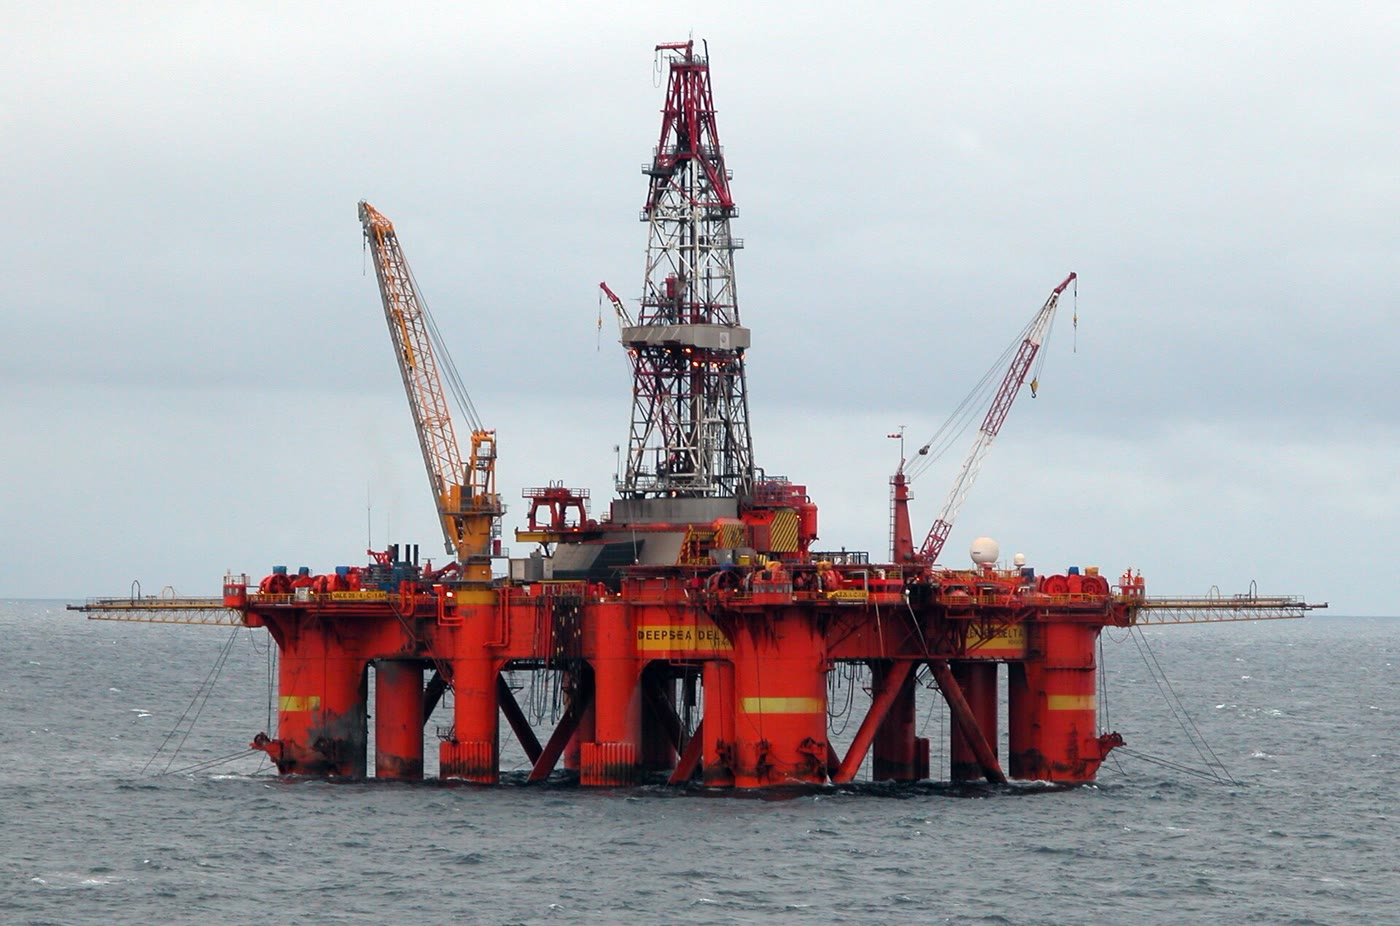
\includegraphics[width=0.66\linewidth]{images/book4/b2-16-drilling-rig.jpg}
\par\smallskip{\small Plate-forme de forage semi-submersible en mer du Nord. Les forages réalisés depuis
de telles plates-formes donnent les épaisseurs, les âges et les types de roches à partir desquels on
reconstitue la subsidence d'un bassin. Photographie Erik Christensen, 2005, CC BY-SA 3.0.}
\end{omfigure}

\section{Bassins et causes de leur enfoncement}\label{sec:b2:basins-compared:types}

Le volume de première année distinguait les bassins par leur position. Ici on les distingue
par ce qui entraîne leur subsidence.

\begin{definition}[Bassins intracratoniques, de rift et de marge passive]\label{def:b2:basins-compared:types}
Un \emph{bassin intracratonique}\index{bassin intracratonique} est un bassin large, rond ou ovale, situé à l'intérieur
d'un continent, loin des limites de plaques, qui s'enfonce lentement pendant de très longues durées
sans faille majeure. Un \emph{bassin de rift}\index{bassin de rift} est un bassin borné par des failles
normales dans une lithosphère continentale qu'on étire~; sa subsidence suit l'étirement, puis le refroidissement
de la lithosphère. Un \emph{bassin de marge passive}\index{bassin de marge passive} est le coin de sédiments,
épaississant vers le large, qui s'accumule sur une marge continentale après la rupture, au-dessus de la croûte amincie
de l'ancien rift.
\end{definition}

Le \omterm{def:b2:alpine-orogen:foreland}{bassin d'avant-pays} du \cref{ch:b2:alpine-orogen} complète la liste, et les bassins qui s'ouvrent
le long de failles de décrochement sont réservés au volume de troisième année. Trois mécanismes font
s'enfoncer le plancher d'un bassin~:
\begin{itemize}
  \item \emph{amincissement} mécanique~: lorsque la croûte est étirée et amincie par des failles, la croûte
        légère est remplacée par du manteau plus dense et la surface s'abaisse pour rétablir l'isostasie~;
  \item \emph{contraction} thermique~: une lithosphère chauffée, par étirement ou par le bas, se refroidit
        ensuite, devient plus dense et s'enfonce, lentement, pendant des dizaines de millions d'années~;
  \item \emph{charge}~: le poids d'une chaîne de chevauchement, ou celui du sédiment lui-même, fait fléchir
        la lithosphère vers le bas~; cette flexion relève du volume de troisième année, et la forme locale,
        d'Airy, de la charge sédimentaire suffit ici.
\end{itemize}
Les \omterm{def:b2:basins-compared:types}{bassins de rift} combinent les deux premiers mécanismes, les marges passives héritent du second de leur
stade de rift, et les \omterm{def:b2:alpine-orogen:foreland}{bassins d'avant-pays} résultent du troisième. Les \omterm{def:b2:basins-compared:types}{bassins intracratoniques} sont les moins bien compris.

\begin{omfigure}
\centering
\begin{tikzpicture}[x=1cm, y=1cm, font=\scriptsize, line join=round,
  sed/.style={fill=yellow!35, draw=black!60, line width=0.3pt},
  crust/.style={fill=orange!25, draw=black!60, line width=0.3pt},
  mlith/.style={fill=green!12, draw=black!60, line width=0.3pt},
  asth/.style={fill=red!12, draw=black!60, line width=0.3pt},
  sea/.style={fill=blue!8, draw=none},
  ttl/.style={anchor=south west, font=\scriptsize\bfseries}]
% (a) intracratonic
\begin{scope}
\fill[asth] (0,-2.4) rectangle (6.6,-1.6);
\fill[mlith] (0,-1.6) rectangle (6.6,-0.7);
\fill[crust] (0,-0.7) -- (6.6,-0.7) -- (6.6,0) -- (4.9,0) .. controls (4.1,-0.45) and (2.5,-0.45) .. (1.7,0) -- (0,0) -- cycle;
\fill[sed] (1.7,0) .. controls (2.5,-0.45) and (4.1,-0.45) .. (4.9,0) -- cycle;
\draw[black!70] (0,0) -- (6.6,0);
\node[ttl] at (0,0.05) {(a) intracratonique};
\node at (3.3,-1.15) {manteau lithosphérique};
\node at (3.3,-2.0) {asthénosphère};
\end{scope}
% (b) rift
\begin{scope}[xshift=7.2cm]
\fill[asth] (0,-2.4) -- (6.6,-2.4) -- (6.6,-1.6) -- (4.5,-1.6) -- (3.3,-1.0) -- (2.1,-1.6) -- (0,-1.6) -- cycle;
\fill[mlith] (0,-1.6) -- (2.1,-1.6) -- (3.3,-1.0) -- (4.5,-1.6) -- (6.6,-1.6) -- (6.6,-0.7) -- (4.4,-0.7) -- (3.3,-0.45) -- (2.2,-0.7) -- (0,-0.7) -- cycle;
\fill[crust] (0,-0.7) -- (2.2,-0.7) -- (3.3,-0.45) -- (4.4,-0.7) -- (6.6,-0.7) -- (6.6,0) -- (4.6,0) -- (4.25,-0.42) -- (3.75,-0.2) -- (3.35,-0.4) -- (2.95,-0.15) -- (2.45,-0.42) -- (2.0,0) -- (0,0) -- cycle;
\fill[sed] (2.0,0) -- (2.45,-0.42) -- (2.95,-0.15) -- (3.35,-0.4) -- (3.75,-0.2) -- (4.25,-0.42) -- (4.6,0) -- cycle;
\draw[thick] (2.0,0) -- (2.5,-0.5) (4.6,0) -- (4.2,-0.5) (2.95,-0.15) -- (3.4,-0.48);
\draw[black!70] (0,0) -- (6.6,0);
\node[ttl] at (0,0.05) {(b) rift};
\node at (1.45,-1.15) {manteau lithosphérique};
\node at (5.4,-2.0) {asthénosphère};
\end{scope}
% (c) passive margin
\begin{scope}[yshift=-3.3cm]
\fill[asth] (0,-2.4) -- (6.6,-2.4) -- (6.6,-1.2) -- (0,-1.6) -- cycle;
\fill[mlith] (0,-1.6) -- (6.6,-1.2) -- (6.6,-1.0) -- (4.2,-1.05) -- (2.4,-0.75) -- (0,-0.7) -- cycle;
\fill[crust] (0,-0.7) -- (2.4,-0.75) -- (4.2,-1.05) -- (4.2,-0.85) -- (2.6,-0.25) -- (1.6,0) -- (0,0) -- cycle;
\fill[gray!35, draw=black!60, line width=0.3pt] (4.2,-1.05) -- (6.6,-1.0) -- (6.6,-0.85) -- (4.2,-0.85) -- cycle;
\fill[sed] (1.6,0) -- (2.6,-0.25) -- (4.2,-0.85) -- (6.6,-0.85) -- (6.6,-0.55) -- (3.6,-0.45) -- (2.6,-0.05) -- (2.2,0) -- cycle;
\fill[sea] (2.2,0) -- (6.6,0) -- (6.6,-0.55) -- (3.6,-0.45) -- (2.6,-0.05) -- cycle;
\draw[black!70] (0,0) -- (2.2,0);
\draw[blue!60!black] (2.2,0) -- (6.6,0);
\node[ttl] at (0,0.05) {(c) marge passive};
\node at (5.4,-0.95) {\tiny croûte océanique};
\node at (1.3,-2.0) {asthénosphère};
\node at (1.3,-1.05) {manteau lithosphérique};
\end{scope}
% (d) foreland
\begin{scope}[xshift=7.2cm, yshift=-3.3cm]
\fill[asth] (0,-2.4) -- (6.6,-2.4) -- (6.6,-2.0) -- (0,-1.5) -- cycle;
\fill[mlith] (0,-1.5) -- (6.6,-2.0) -- (6.6,-1.2) -- (0,-0.7) -- cycle;
\fill[crust] (0,-0.7) -- (6.6,-1.2) -- (6.6,-0.55) -- (3.6,-0.4) .. controls (2.0,-0.15) .. (0,0) -- cycle;
\fill[sed] (0,0) .. controls (2.0,-0.15) .. (3.6,-0.4) -- (6.6,-0.55) -- (5.0,0) -- cycle;
\fill[crust, fill=orange!45] (5.0,0) -- (6.6,-0.55) -- (6.6,0.6) -- (6.1,0.6) -- cycle;
\draw[thrust fault] (6.6,-0.55) -- (5.0,0);
\draw[black!70] (0,0) -- (5.0,0);
\node[ttl] at (0,0.05) {(d) avant-pays};
\node[anchor=north east, font=\tiny] at (6.55,0.55) {chaîne};
\node at (2.2,-1.25) {manteau lithosphérique};
\node at (1.5,-2.05) {asthénosphère};
\end{scope}
\end{tikzpicture}
\par\smallskip{\small Quatre familles de bassins, en coupes schématiques à travers la lithosphère (non
à l'échelle~; sédiment en jaune, croûte continentale en orange, croûte océanique en gris). L'exagération
verticale est grande~: les bassins réels ont des centaines de kilomètres de large et quelques à quinze kilomètres
de profondeur.}
\end{omfigure}

Les \omterm{def:b2:basins-compared:types}{bassins de rift} de la mer du Nord sont le cas classique des deux premiers mécanismes. Des grabens
s'y sont formés dès le Trias, et le dernier étirement majeur a duré du Jurassique moyen au Crétacé moyen ; les failles
se sont ensuite tues, et le centre du bassin a continué de s'enfoncer en cuvette large, comblée par des craies,
des grès et, pendant la plus grande partie du Tertiaire, des schistes et des argilites. Chargé par l'eau seule,
son socle se serait enfoncé encore de 1100 à \qty{1400}{m} au centre et de 600 à \qty{700}{m} sur les flancs
après l'arrêt des failles.
% ledger: sc80b4:north-sea

La marge passive de la côte est des États-Unis montre le même enfoncement, à plus grande échelle.
Les profils sismiques à travers le plateau montrent plus de \qty{14}{km} de roches mésozoïques et plus récentes dans
le Baltimore Canyon Trough, et \qty{8}{km} dans le bassin de Georges Bank, en couches qui s'épaississent vers le large.
Ses dépocentres jurassiques suivent les structures du rift et les zones de sa subsidence
thermique ultérieure.
% ledger: schlee76:atlantic, lang24:atlantic

Le bassin du Michigan est le type des \omterm{def:b2:basins-compared:types}{bassins intracratoniques}. De forme ovale, il couvre quelques centaines de milliers
de kilomètres carrés et renferme plus de \qty{4}{km} de sédiments phanérozoïques, déposés en épisodes distincts
pendant quelque 500 millions d'années, avec peu de failles. Ses épisodes de subsidence plus rapide coïncident avec ceux
d'autres bassins situés à l'intérieur de l'Amérique du Nord et d'autres continents, ce qui suggère une cause plus vaste
qu'un seul bassin. Le \omterm{def:b2:basins-compared:backstripping}{backstripping} de plus de 57\,000 diagraphies de puits montre une subsidence
durable et presque circulaire, que les auteurs suggèrent pouvoir attribuer à un flux descendant du manteau,
interrompue aux époques de deux orogenèses sur la marge lointaine du continent. Pourquoi
les \omterm{def:b2:basins-compared:types}{bassins intracratoniques} s'enfoncent reste un sujet de débat.
% ledger: sloss82:michigan, crowe09:michigan

\section{Courbes de subsidence}\label{sec:b2:basins-compared:curves}

Un puits, ou une coupe mesurée, donne pour chaque unité sa profondeur actuelle, son type de roche et son âge,
lu sur des fossiles ou par corrélation. Avec la profondeur d'eau dans laquelle chaque unité s'est déposée,
lue sur ses fossiles et ses structures sédimentaires, il donne l'histoire du bassin.

\begin{definition}[Courbe de subsidence]\label{def:b2:basins-compared:curve}
Une \emph{courbe de subsidence}\index{courbe de subsidence} d'un bassin en un site est le graphe de la profondeur
d'une surface de référence, en général le socle ou la base de l'unité la plus ancienne, sous le niveau de la mer,
en fonction du temps. La courbe de subsidence \emph{totale} utilise l'épaisseur du sédiment telle qu'elle était à chaque
époque, plus la profondeur d'eau~; la courbe de subsidence \emph{tectonique} remplace le sédiment par de l'eau et
supprime son effet isostatique.
\end{definition}

Une unité n'a jamais été aussi épaisse dans le passé qu'aujourd'hui. Enfouie, elle a perdu sa porosité~: ses grains
n'ont pas changé, mais leur eau a été expulsée. Le volume de première année écrivait la porosité à la profondeur
$z$ sous la forme de la loi d'Athy, $\phi(z) = \phi_0\,e^{-z/c}$, et trouvait l'épaisseur solide d'une couche comprise entre
$z_1$ et $z_2$,
\[
  T_s = (z_2 - z_1) - \phi_0 c\left(e^{-z_1/c} - e^{-z_2/c}\right),
\]
qui reste la même lorsque la couche se déplace. Pour \emph{décompacter} une unité jusqu'à une position moins profonde,
son sommet étant désormais en $z_1'$, on cherche la base $z_2'$ qui conserve la même épaisseur solide. L'équation
n'a pas de solution fermée, mais l'itération de point fixe
\[
  z_2' \leftarrow z_1' + T_s + \phi_0 c\left(e^{-z_1'/c} - e^{-z_2'/c}\right)
\]
à partir de $z_2' = z_1' + T_s$ converge en quelques pas. La masse par unité de surface de la couche
est celle de ses grains plus celle de son eau interstitielle,
\[
  m = \rho_g T_s + \rho_w\,(z_2 - z_1 - T_s),
\]
avec $\rho_g$ la masse volumique des grains~; diviser la masse d'une colonne par son épaisseur donne
sa masse volumique moyenne $\bar\rho_s$.

Pour les lithologies de ce chapitre, sable, argilite, craie et sable argileux, le tableau ci-dessous donne
les constantes de Sclater et Christie (1980), telles qu'elles sont regroupées dans un programme libre. Le sable
garde sa porosité le plus profondément, la craie la perd le plus vite.
% ledger: pybacktrack:compaction

\begin{center}
\small
\begin{tabular}{lccc}
\hline
lithologie & densité des grains (\unit{kg.m^{-3}}) & porosité de surface $\phi_0$ & longueur de décroissance $c$ (\unit{m}) \\
\hline
sable & 2650 & 0.49 & 3704 \\
argilite & 2700 & 0.63 & 1960 \\
craie & 2710 & 0.70 & 1408 \\
sable argileux & 2680 & 0.56 & 2564 \\
\hline
\end{tabular}
\end{center}

\section{Backstripping (décompaction-désurcharge)}\label{sec:b2:basins-compared:backstripping}

Une \omterm{def:b2:basins-compared:curve}{courbe de subsidence} totale mêle deux causes~: ce qui a fait le bassin, et le poids de ce qui
l'a rempli. Les séparer est l'objet de la procédure suivante, l'outil central de
l'analyse de bassin.

\begin{definition}[Backstripping]\label{def:b2:basins-compared:backstripping}
\emph{Backstripping}\index{backstripping} est la reconstruction de la subsidence tectonique d'un bassin au cours du temps~:
les unités d'un puits sont retirées une à une, en commençant par la plus jeune~; les unités restantes sont décompactées
à chaque étape, et l'effet isostatique de la charge sédimentaire et de l'eau est retiré pour donner la profondeur
à laquelle le socle se serait tenu sous l'eau seule.
\end{definition}

La dernière étape est un bilan isostatique. Le volume de première année l'a établi pour un bassin rempli jusqu'au niveau de la mer~;
le cas général ajoute la profondeur d'eau et le niveau de la mer.

\begin{proposition}[Backstripping d'Airy]\label{prop:b2:basins-compared:backstrip}
Soit un bassin qui porte, à un instant donné, une colonne de sédiment d'épaisseur $S$ et de masse volumique moyenne
$\bar\rho_s$, sous une profondeur d'eau $W_d$, alors que la mer se tenait $\Delta_{SL}$ au-dessus de son niveau actuel.
En isostasie locale au-dessus d'un manteau de masse volumique $\rho_m$, avec de l'eau de masse volumique $\rho_w$, la
subsidence tectonique à cet instant, mesurée depuis le niveau actuel de la mer, vaut
\[
  Y = S\,\frac{\rho_m - \bar\rho_s}{\rho_m - \rho_w} + W_d
      - \Delta_{SL}\,\frac{\rho_m}{\rho_m - \rho_w}.
\]
\end{proposition}

\begin{proof}
Comparons deux colonnes posées sur la même lithosphère, jusqu'à une profondeur de compensation située sous les deux. Dans
la première, une eau de profondeur $W_d$ recouvre le sédiment d'épaisseur $S$~; dans la seconde, l'eau seule
remplit un bassin de profondeur $Y'$ sous la même surface de la mer. Leurs masses sont égales~:
\[
  \rho_w W_d + \bar\rho_s S + \rho_m\,(d - W_d - S) = \rho_w Y' + \rho_m\,(d - Y'),
\]
avec $d$ la profondeur commune de la compensation sous la surface de la mer. D'où
$Y'(\rho_m - \rho_w) = S(\rho_m - \bar\rho_s) + W_d(\rho_m - \rho_w)$, ce qui donne les deux premiers
termes. Si la mer se tenait $\Delta_{SL}$ plus haut qu'aujourd'hui, cette eau supplémentaire ne fait pas partie de la
subsidence propre du bassin~: en la retirant, le socle chargé d'eau remonte de
$\Delta_{SL}\rho_w/(\rho_m - \rho_w)$, et sa profondeur sous le niveau actuel de la mer diminue encore de
$\Delta_{SL}$~; au total, $\Delta_{SL}\,\rho_m/(\rho_m - \rho_w)$.
\end{proof}
% ledger: pybacktrack:backstrip

Avec $\rho_m = \qty{3330}{kg.m^{-3}}$ et $\rho_w = \qty{1030}{kg.m^{-3}}$, une colonne de sédiment de masse volumique
moyenne \qty{2300}{kg.m^{-3}} compte pour $1030/2300 = 0.45$ de son épaisseur dans la subsidence
tectonique~: plus de la moitié de l'épaisseur du remplissage d'un bassin est de la place créée par son propre poids.
Une mer \qty{100}{m} plus haute qu'aujourd'hui abaisse le résultat de \qty{145}{m}. La profondeur d'eau et le niveau
passé de la mer sont les données les plus faibles~: les fossiles donnent une fourchette de profondeurs d'eau, souvent large de
centaines de mètres sur la pente, et la subsidence tectonique en hérite.

\begin{method}[Backstripping d'un puits]\label{met:b2:basins-compared:backstrip}
\begin{enumerate}
  \item Lister les unités depuis la base, avec les profondeurs actuelles de leurs sommets et de leurs bases, leurs
        constantes lithologiques $(\rho_g, \phi_0, c)$, les âges de leurs sommets, et la profondeur d'eau à
        chacun de ces âges.
  \item Calculer l'épaisseur solide $T_s$ de chaque unité à partir de ses profondeurs actuelles.
  \item Pour l'âge du sommet de l'unité $k$, retirer toutes les unités plus jeunes. Placer le sommet de l'unité
        $k$ à profondeur nulle et la décompacter~; placer chaque unité plus ancienne, à son tour, sous celle qui la
        surmonte, et la décompacter.
  \item Additionner les épaisseurs pour obtenir $S$, et les masses pour obtenir la masse volumique moyenne
        $\bar\rho_s = \sum m / S$.
  \item Appliquer la \cref{prop:b2:basins-compared:backstrip} pour obtenir $Y$~; la subsidence totale vaut
        $S + W_d$.
  \item Répéter pour chaque âge, du plus ancien au présent~; tracer $Y$ et $S + W_d$ en fonction de l'âge.
\end{enumerate}
\end{method}

La figure ci-dessous montre le résultat pour un puits fictif dans un \omterm{def:b2:basins-compared:types}{bassin de rift}. Quatre unités ont été carottées~:
un sable syn-rift déposé pendant que les failles étaient actives, entre 165 et \qty{150}{Ma}~; puis une argilite,
une craie et un sable argileux. Aujourd'hui, aucune décompaction n'est nécessaire~: le socle se trouve à \qty{6030}{m}
et la colonne a une masse volumique moyenne de \qty{2358}{kg.m^{-3}}, de sorte que $Y = \qty{2648}{m}$ sous
\qty{100}{m} d'eau. À \qty{150}{Ma}, le seul sable, décompacté à la surface, mesurait
\qty{2239}{m} d'épaisseur, avec une masse volumique moyenne de \qty{2055}{kg.m^{-3}}~: sous \qty{200}{m} d'eau,
$Y = \qty{1441}{m}$. La subsidence totale vaut
plus du double de la subsidence tectonique, et la courbe tectonique montre un premier stade rapide, puis
un enfoncement qui ralentit~: la forme d'un rift.
% values (script): figdata/bachelor-2/basins.py part numbers (S_150 2239.5, rho_0 2357.9, Y_0 2648.7, Y_150 1442.1); printed from the rounded chain of calc/ch16.py (rho 2358 -> 2648; T 2239, rho 2055 -> 1441), as in the problem

\begin{omfigure}
\centering
% figdata/bachelor-2/basins.py parts stages and fit (invented well)
\begin{tikzpicture}
\begin{axis}[width=0.8\linewidth, height=6.0cm, x dir=reverse, y dir=reverse, xmin=0, xmax=170,
  ymin=0, ymax=6500, xlabel={âge (\unit{Ma})}, ylabel={profondeur sous le niveau de la mer (\unit{m})},
  tick label style={font=\scriptsize}, label style={font=\small}, xtick={0,25,...,175},
  xtick pos=bottom, ytick pos=left,
  legend style={at={(0.5,1.04)}, anchor=south, draw=none, font=\scriptsize, legend columns=3,
  /tikz/every even column/.append style={column sep=8pt}}]
\addplot[omThm, line width=1pt, mark=*, mark size=1.6pt] table[x=age_Ma, y=total_m]
  {figdata/out/bachelor-2-basins-stages.dat};
\addlegendentry{subsidence totale $S + W_d$}
\addplot[blue!70!black, line width=1pt, mark=square*, mark size=1.6pt] table[x=age_Ma, y=Y_m]
  {figdata/out/bachelor-2-basins-stages.dat};
\addlegendentry{subsidence tectonique $Y$}
\addplot[black!70, dashed, line width=0.8pt] table[x=age_Ma, y=Y_m]
  {figdata/out/bachelor-2-basins-fit.dat};
\addlegendentry{modèle d'étirement, $\beta = 1.50$}
\node[font=\scriptsize, anchor=south west] at (axis cs:149,1500) {fin du rifting};
\end{axis}
\end{tikzpicture}
\par\smallskip{\small \omterm{def:b2:basins-compared:backstripping}{Backstripping} d'un puits fictif à quatre unités (données dans le
problème du week-end)~: profondeur du socle avec le sédiment tel qu'il était à chaque époque, et subsidence
tectonique, avec la courbe du \omterm{def:b2:basins-compared:stretching}{modèle d'étirement} ajustée à la subsidence en fin de rifting
(\cref{sec:b2:basins-compared:stretching}).}
\end{omfigure}

\begin{omfigure}
\centering
\begin{tikzpicture}[x=1cm, y=0.1cm, font=\scriptsize, line join=round,
  u/.style={draw=black!60, line width=0.3pt}]
% today
\begin{scope}
\fill[blue!8] (0,0) rectangle (1.6,-1.0);
\fill[u, fill=yellow!25] (0,-1.0) rectangle (1.6,-18.0);
\fill[u, fill=green!18] (0,-18.0) rectangle (1.6,-34.1);
\fill[u, fill=gray!25] (0,-34.1) rectangle (1.6,-45.2);
\fill[u, fill=yellow!55] (0,-45.2) rectangle (1.6,-61.3);
\draw[black!70] (0,-61.3) -- (1.6,-61.3);
\node[anchor=south] at (0.8,0.1) {aujourd'hui};
\node at (0.8,-9.5) {sable argileux};
\node at (0.8,-26) {craie};
\node at (0.8,-39.6) {argilite};
\node at (0.8,-53.2) {sable};
\node[anchor=north] at (0.8,-61.5) {\qty{6130}{m}};
\end{scope}
% at 150 Ma
\begin{scope}[xshift=3.0cm]
\fill[blue!8] (0,0) rectangle (1.6,-2.0);
\fill[u, fill=yellow!55] (0,-2.0) rectangle (1.6,-24.39);
\draw[black!70] (0,-24.4) -- (1.6,-24.4);
\node[anchor=south] at (0.8,0.1) {\qty{150}{Ma}};
\node at (0.8,-13.2) {sable};
\node[anchor=north] at (0.8,-24.6) {\qty{2439}{m}};
\end{scope}
\draw[-{Latex}, thick] (4.9,-12) -- (6.1,-12) node[midway, above] {allègement};
% water loaded
\begin{scope}[xshift=6.3cm]
\fill[blue!20] (0,0) rectangle (1.6,-14.4);
\draw[black!70] (0,-14.4) -- (1.6,-14.4);
\node[anchor=south] at (0.8,0.1) {eau seule};
\node at (0.8,-7.2) {eau};
\node[anchor=north] at (0.8,-14.6) {$Y = \qty{1441}{m}$};
\end{scope}
\draw[black!40, dashed] (-0.3,0) -- (8.2,0);
\node[anchor=west] at (8.2,0) {niveau de la mer};
\end{tikzpicture}
\par\smallskip{\small \omterm{def:b2:basins-compared:backstripping}{Backstripping} du puits fictif à \qty{150}{Ma} (profondeurs à l'échelle)~: les quatre unités
aujourd'hui~; le seul sable en fin de rift, décompacté à la surface
sous \qty{200}{m} d'eau~; la même lithosphère chargée par l'eau seule, dont le socle se tient plus haut
parce que l'eau est plus légère que le sédiment.}
\end{omfigure}

\section{Le modèle d'étirement}\label{sec:b2:basins-compared:stretching}

Pourquoi un \omterm{def:b2:basins-compared:types}{bassin de rift} s'enfonce-t-il d'abord vite, puis lentement~? En 1978, D. McKenzie a proposé un modèle si
simple que ses paramètres peuvent être ajustés sur un seul puits.

\begin{definition}[Modèle d'étirement ; facteur d'étirement ; subsidence syn-rift et post-rift]\label{def:b2:basins-compared:stretching}
Le \emph{modèle d'étirement}\index{modèle d'étirement} d'un bassin représente le rifting comme un
étirement instantané et uniforme de toute la lithosphère par cisaillement pur : croûte et manteau
lithosphérique sont amincis du même facteur, et l'asthénosphère chaude remonte passivement pour remplir
l'espace, après quoi la lithosphère se refroidit. Le \emph{facteur d'étirement}\index{facteur d'étirement}
$\beta$ est le rapport de la largeur de la région étirée après étirement à sa largeur avant,
égal au rapport de l'épaisseur initiale à l'épaisseur finale de la croûte. La subsidence produite
pendant l'étirement est la \emph{subsidence syn-rift}\index{subsidence syn-rift}~; celle qui suit,
due au refroidissement de la lithosphère, est la \emph{subsidence
post-rift}\index{subsidence post-rift}, ou subsidence thermique.
\end{definition}

L'étirement dans la nature dure un temps fini, de quelques millions d'années. Les versions ultérieures du modèle le laissent
durer, mais tant qu'il n'est pas trop lent, la version instantanée simple donne la subsidence à peu près, mais correctement,
puisque après l'étirement le refroidissement se déroule à peu près de la même façon.
% ledger: sheplev98:model

\begin{omfigure}
\centering
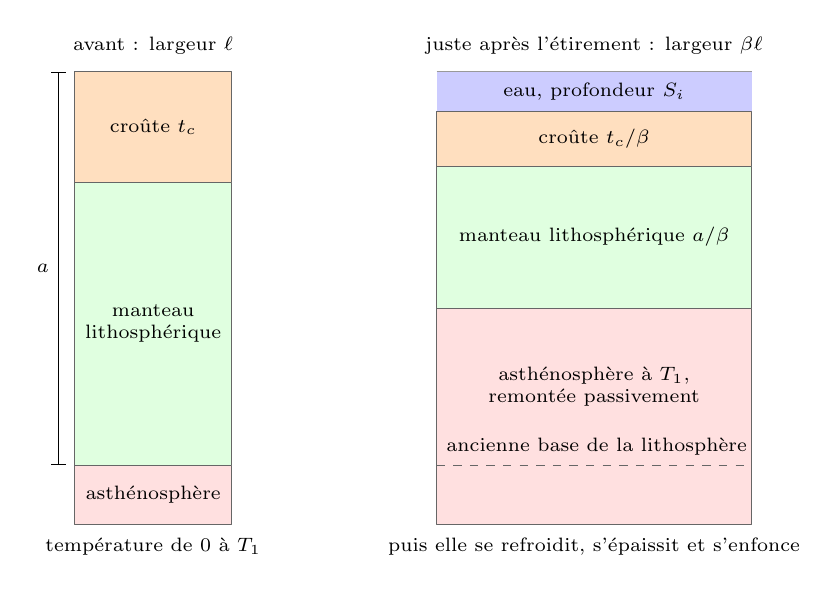
\begin{tikzpicture}[x=0.5cm, y=0.5cm, font=\scriptsize, line join=round]
% before
\begin{scope}
\fill[orange!25, draw=black!60, line width=0.3pt] (0,0) rectangle (4,-2.8);
\fill[green!12, draw=black!60, line width=0.3pt] (0,-2.8) rectangle (4,-10);
\fill[red!12, draw=black!60, line width=0.3pt] (0,-10) rectangle (4,-11.5);
\node at (2,-1.4) {croûte $t_c$};
\node[align=center] at (2,-6.4) {manteau\\lithosphérique};
\node at (2,-10.75) {asthénosphère};
\draw[|-|] (-0.4,0) -- (-0.4,-10) node[midway, left] {$a$};
\node[anchor=south] at (2,0.2) {avant : largeur $\ell$};
\node[anchor=north] at (2,-11.6) {température de $0$ à $T_1$};
\end{scope}
% after
\begin{scope}[xshift=4.6cm]
\fill[blue!20] (0,0) rectangle (8,-1.0);
\fill[orange!25, draw=black!60, line width=0.3pt] (0,-1.0) rectangle (8,-2.4);
\fill[green!12, draw=black!60, line width=0.3pt] (0,-2.4) rectangle (8,-6.0);
\fill[red!12, draw=black!60, line width=0.3pt] (0,-6.0) rectangle (8,-11.5);
\draw[black!60, dashed] (0,-10) -- (8,-10);
\node at (4,-0.5) {eau, profondeur $S_i$};
\node at (4,-1.7) {croûte $t_c/\beta$};
\node at (4,-4.2) {manteau lithosphérique $a/\beta$};
\node[align=center] at (4,-8.0) {asthénosphère à $T_1$,\\remontée passivement};
\node[anchor=south west] at (0,-10) {ancienne base de la lithosphère};
\node[anchor=south] at (4,0.2) {juste après l'étirement : largeur $\beta\ell$};
\node[anchor=north] at (4,-11.6) {puis elle se refroidit, s'épaissit et s'enfonce};
\draw[black!40] (0,0) -- (8,0);
\end{scope}
\end{tikzpicture}
\par\smallskip{\small Le \omterm{def:b2:basins-compared:stretching}{modèle d'étirement} (non à l'échelle) : une lithosphère d'épaisseur $a$ avec une
croûte $t_c$ est étirée à $\beta$ fois sa largeur~; croûte et manteau lithosphérique s'amincissent de
$\beta$, l'asthénosphère remonte, et la surface s'enfonce de la \omterm{def:b2:basins-compared:stretching}{subsidence syn-rift} $S_i$ sous
l'eau. Ici $\beta = 2$.}
\end{omfigure}

\begin{proposition}[Subsidence dans le modèle d'étirement]\label{prop:b2:basins-compared:stretching}
Soit une lithosphère d'épaisseur $a$, avec une croûte d'épaisseur $t_c$, dont le géotherme est linéaire, de
$0$ en surface à la température $T_1$ de l'asthénosphère à sa base~; soient croûte et manteau de masses volumiques
$\rho_c(1 - \alpha T)$ et $\rho_m(1 - \alpha T)$, avec $\alpha$ le coefficient de dilatation thermique. Si elle est étirée
instantanément de $\beta$ et que le bassin est rempli
d'eau de masse volumique $\rho_w$~:
\begin{enumerate}
  \item la \omterm{def:b2:basins-compared:stretching}{subsidence syn-rift} vaut
  \[
    S_i = \frac{a\left(1 - \dfrac{1}{\beta}\right)\left[(\rho_m - \rho_c)\dfrac{t_c}{a}
          \left(1 - \dfrac{\alpha T_1 t_c}{2a}\right) - \dfrac{\alpha T_1 \rho_m}{2}\right]}
          {\rho_m(1 - \alpha T_1) - \rho_w};
  \]
  \item la \omterm{def:b2:basins-compared:stretching}{subsidence post-rift}, à un temps $t$ après l'étirement, vaut, au premier terme d'une série,
  \[
    S_t = E_0\,\frac{\beta}{\pi}\sin\frac{\pi}{\beta}\left(1 - e^{-t/\tau}\right),\qquad
    E_0 = \frac{4a\rho_m\alpha T_1}{\pi^2(\rho_m - \rho_w)},\qquad
    \tau = \frac{a^2}{\pi^2\kappa},
  \]
où $\kappa$ est la diffusivité thermique et $\tau$ la \emph{constante de temps
thermique}\index{constante de temps thermique} de la lithosphère.
\end{enumerate}
\end{proposition}
% ledger: pybacktrack:rifting

\begin{proof}
(1) Comparons la colonne avant l'étirement à la colonne juste après, jusqu'à l'ancienne base de la lithosphère,
à la profondeur $a$ sous la surface avant l'étirement. Avant, la croûte d'épaisseur $t_c$ et le manteau
lithosphérique sont à des températures $T = T_1 z/a$~; après, les deux sont amincis d'un facteur $\beta$,
et leurs températures vont de $0$ à $T_1$ sur $a/\beta$, de sorte qu'un point situé à la profondeur $z'$ sous la base
de l'eau a $T = T_1\beta z'/a$~; dessous, l'asthénosphère à $T_1$ a une masse volumique $\rho_m(1 - \alpha T_1)$~;
au-dessus, l'eau remplit la profondeur $S_i$. La masse d'une couche de masse volumique $\rho(1 - \alpha T)$
dans laquelle $T$ croît linéairement de $T_a$ à $T_b$ vaut $\rho\,h\,(1 - \alpha(T_a + T_b)/2)$.
Avant, la colonne contient
\[
  \rho_c t_c\left(1 - \frac{\alpha T_1 t_c}{2a}\right)
  + \rho_m (a - t_c)\left(1 - \frac{\alpha T_1 (a + t_c)}{2a}\right);
\]
après, elle contient l'eau, la croûte et le manteau lithosphérique amincis, et l'asthénosphère qui
remplit le reste de la profondeur $a$~:
\[
  \rho_w S_i + \frac{\rho_c t_c}{\beta}\left(1 - \frac{\alpha T_1 t_c}{2a}\right)
  + \frac{\rho_m (a - t_c)}{\beta}\left(1 - \frac{\alpha T_1 (a + t_c)}{2a}\right)
  + \rho_m(1 - \alpha T_1)\left(a - S_i - \frac{a}{\beta}\right).
\]
L'isostasie égalise les deux. En rassemblant les termes en $S_i$ d'un côté et le facteur
$(1 - 1/\beta)$ de l'autre, et en développant, on obtient la formule~; le calcul est
\cref{exo:b2:basins-compared:11}.

(2) Après l'étirement, la plaque se refroidit par conduction entre une surface maintenue à $0$ et une base maintenue
à $T_1$, vers le profil linéaire dont elle est partie. L'excès de température résout l'équation de la chaleur
avec des valeurs nulles au sommet et à la base, et s'écrit donc comme une somme de termes
$b_n\sin(n\pi z/a)\,e^{-n^2\kappa\pi^2 t/a^2}$~; chacun se refroidit avec son propre temps, $\tau/n^2$. La chaleur perdue
fait contracter la colonne de $\alpha\int \Delta T\,\mathrm{d}z$, et l'eau supplémentaire qui remplit l'espace l'enfonce encore
du facteur $\rho_m/(\rho_m - \rho_w)$. Seuls les termes impairs contribuent~; en gardant le premier, dont le coefficient
se calcule à partir du profil initial, donne l'expression. Les autres se refroidissent neuf fois ou plus vite,
et après une dizaine de millions d'années, ils décalent la subsidence d'une quantité presque constante, inférieure
à \qty{100}{m} pour $\beta$ compris entre 1.2
et 4, avec les valeurs ci-dessous.
\end{proof}
% values (script): basins.thermal_series vs basins.thermal, tested in tests/bachelor-2/test_basins.py

Les paramètres de l'article de McKenzie sont $a = \qty{125}{km}$, $T_1 = \qty{1333}{\celsius}$,
$\alpha = \qty{3.28e-5}{K^{-1}}$, $\kappa = \qty{8e-7}{m^2.s^{-1}}$, $\rho_m =
\qty{3330}{kg.m^{-3}}$ (à \qty{0}{\celsius}), $\rho_c = \qty{2800}{kg.m^{-3}}$~; avec de l'eau de mer à
\qty{1030}{kg.m^{-3}} elles donnent $\tau = \qty{62.7}{Ma}$ et $E_0 = \qty{3207}{m}$. Avec une croûte de
\qty{35}{km}, la \omterm{def:b2:basins-compared:stretching}{subsidence syn-rift} vaut $S_i = \qty{4334}{m} \times (1 - 1/\beta)$.
% ledger: sheplev98:parameters, pybacktrack:rifting
% values (script): tau_Myr 62.7, E0_m 3206.9, Si_max_m 4333.8

\begin{omfigure}
\centering
% figdata/bachelor-2/basins.py part curves
\begin{tikzpicture}
\begin{axis}[width=0.8\linewidth, height=6.2cm, y dir=reverse, xmin=0, xmax=200, ymin=0,
  ymax=6500, xlabel={temps après l'étirement (\unit{Ma})},
  ylabel={subsidence tectonique (\unit{m})}, tick label style={font=\scriptsize},
  label style={font=\small}, xtick pos=bottom, ytick pos=left]
\addplot[black!45, line width=1pt] table[x=t_Myr, y=b1.2] {figdata/out/bachelor-2-basins-curves.dat};
\addplot[blue!70!black, line width=1pt] table[x=t_Myr, y=b1.5] {figdata/out/bachelor-2-basins-curves.dat};
\addplot[omThm, line width=1pt] table[x=t_Myr, y=b2] {figdata/out/bachelor-2-basins-curves.dat};
\addplot[orange!80!black, line width=1pt] table[x=t_Myr, y=b4] {figdata/out/bachelor-2-basins-curves.dat};
\node[font=\scriptsize, anchor=south west, inner sep=1pt] at (axis cs:150,1225) {$\beta = 1.2$};
\node[font=\scriptsize, anchor=south west, inner sep=1pt] at (axis cs:150,2595) {$\beta = 1.5$};
\node[font=\scriptsize, anchor=south west, inner sep=1pt] at (axis cs:150,3965) {$\beta = 2$};
\node[font=\scriptsize, anchor=south west, inner sep=1pt] at (axis cs:150,5815) {$\beta = 4$};
\draw[black!40, dashed] (axis cs:62.7,0) -- (axis cs:62.7,6500);
\node[font=\scriptsize, anchor=north west] at (axis cs:63,150) {$t = \tau$};
\end{axis}
\end{tikzpicture}
\par\smallskip{\small Subsidence à charge d'eau du \omterm{def:b2:basins-compared:stretching}{modèle d'étirement} pour quatre \omterm{def:b2:basins-compared:stretching}{facteurs d'étirement},
avec une croûte de \qty{35}{km} et les paramètres du texte~: le pas syn-rift à
$t = 0$, puis la courbe post-rift, qui a atteint \qty{63}{\percent} de sa valeur finale à
$t = \tau$.}
\end{omfigure}

Trois caractéristiques du modèle se transposent aux bassins réels.
\begin{itemize}
  \item La marche syn-rift croît avec $\beta$, et la \omterm{def:b2:basins-compared:stretching}{subsidence post-rift} aussi~; mais leur rapport
        change peu, de sorte que les deux parties indiquent le même $\beta$ si le modèle est valable.
  \item L'échelle de temps de la \omterm{def:b2:basins-compared:stretching}{subsidence post-rift} ne dépend pas de $\beta$~: elle est fixée par l'épaisseur
        de la lithosphère seule. Après $\tau$, \qty{63}{\percent} de la subsidence thermique est acquise~; après
        $3\tau$, environ \qty{95}{\percent}. Un rift arrêté il y a deux cents millions d'années
        ne s'enfonce presque plus.
  \item Le terme syn-rift est une compétition entre la croûte légère amincie, qui fait s'enfoncer la surface, et
        l'asthénosphère chaude remontée, qui la soutient. Avec une croûte mince, la seconde l'emporte et l'étirement
        élève la surface (\cref{exo:b2:basins-compared:10}).
\end{itemize}

Pour ajuster un puits, la subsidence tectonique en fin de rifting donne $S_i$, donc
$\beta = 1/(1 - S_i/\qty{4334}{m})$ pour une croûte de \qty{35}{km}~; la courbe post-rift est alors prédite
et comparée aux autres points backstrippés. Dans le puits fictif, $S_i = \qty{1441}{m}$
donne $\beta = 1.50$, et la courbe passe à quelques mètres des points plus récents (figure de
\cref{sec:b2:basins-compared:backstripping}). Les bassins réels se prêtent rarement si bien à l'exercice.
En mer du Nord centrale, un étirement de 50 à \qty{100}{\percent} au milieu, avec $\beta$ de 1.5 à 2, reproduit l'amplitude
et la vitesse de la \omterm{def:b2:basins-compared:stretching}{subsidence post-rift}. Sur la marge orientale des États-Unis,
seul un segment, la plate-forme de Long Island, a un remplissage post-rift précoce aussi épais que le prévoit
un étirement uniforme~; dans le Georges Bank Basin et le Baltimore Canyon Trough, le remplissage est
1.5 à 3 fois plus épais, et d'autres causes doivent agir.
% ledger: sc80b4:north-sea, lang24:atlantic

\section{Bassins comparés}\label{sec:b2:basins-compared:compared}

Le tableau ci-dessous rassemble les quatre familles. Les courbes diffèrent par leur forme et leur échelle de temps, et une \omterm{def:b2:basins-compared:curve}{courbe de
subsidence} est souvent le premier indice de la nature d'un bassin enfoui sous des roches plus récentes.

\begin{center}
\small
\begin{tabular}{>{\raggedright\arraybackslash}p{0.13\linewidth}>{\raggedright\arraybackslash}p{0.19\linewidth}>{\raggedright\arraybackslash}p{0.26\linewidth}>{\raggedright\arraybackslash}p{0.29\linewidth}}
\hline
bassin & exemple & épaisseur et durée & forme de la \omterm{def:b2:basins-compared:curve}{courbe de subsidence} tectonique \\
\hline
rift & centre de la mer du Nord & grabens depuis le Trias~; dernier étirement du Jurassique moyen au
Crétacé moyen~; de 1.1 à \qty{1.4}{km} d'enfoncement post-rift sous charge d'eau & une marche syn-rift rapide,
puis un ralentissement exponentiel, avec $\tau$ de dizaines de Ma \\
marge passive & Baltimore Canyon Trough & plus de \qty{14}{km} depuis le Jurassique & comme un rift,
avec une grande part post-rift~; le remplissage s'épaissit vers le large \\
avant-pays & \omterm{def:b2:alpine-orogen:foreland}{molasse} nord-alpine & plus de \qty{4}{km} au front de chevauchement, de l'Éocène supérieur au
Miocène supérieur & le plus profond contre la chaîne, en migrant avec elle~; sa partie interne finalement
recouverte par les chevauchements \\
intra\-cratonique & Michigan & plus de \qty{4}{km} par épisodes sur quelque 500 Ma & lente, avec des
épisodes d'enfoncement plus rapide communs à des bassins éloignés \\
\hline
\end{tabular}
\end{center}
% ledger: sc80b4:north-sea, schlee76:atlantic, poag79:bct, krenmayr99:molasse, schmid04:foreland, sloss82:michigan

Un \omterm{def:b2:alpine-orogen:foreland}{bassin d'avant-pays} s'enfonce sous une charge qui se déplace vers lui~: le bassin migre avec la chaîne,
le bassin alpin, d'au moins \qty{210}{km} sur le craton européen, et sa partie interne est finalement
recouverte et entraînée par les chevauchements, comme la \omterm{def:b2:alpine-orogen:foreland}{molasse} subalpine l'a été dans
\cref{ch:b2:alpine-orogen}. Un rift ralentit en se refroidissant, quel que soit son étirement~;
un \omterm{def:b2:basins-compared:types}{bassin intracratonique} s'enfonce lentement et longtemps, par pulsations~; ni l'étirement
ni une charge n'en rendent bien compte, ce qui en fait encore une question de recherche.
% ledger: schmid04:foreland, sinclair97:trinity, krenmayr99:molasse

\begin{inthelab}[Analyse de la subsidence]
Les analystes de bassin font avec des programmes le travail de la méthode. Un programme libre, par exemple, lit
un site de forage comme une liste d'unités, avec leurs âges, leurs profondeurs et leurs lithologies, ainsi qu'une table
des lithologies avec leur masse volumique des grains, leur porosité de surface et leur longueur de décroissance. Son
module de \omterm{def:b2:basins-compared:backstripping}{backstripping} décompacte les unités et renvoie la subsidence tectonique à chaque âge~;
puisqu'une profondeur d'eau ancienne n'est connue que sous forme d'intervalle, l'utilisateur donne un minimum et un maximum, et
le programme renvoie les deux subsidences et leur moyenne. Un second module travaille dans l'autre sens~:
à partir d'un modèle de subsidence tectonique, il prédit les profondeurs d'eau du passé, que l'on peut
confronter aux fossiles. Les analystes ajustent ensuite des \omterm{def:b2:basins-compared:stretching}{facteurs d'étirement}, testent des courbes du niveau marin et
cartographient la subsidence d'un bassin entier à partir de centaines ou de milliers de puits.
\end{inthelab}
% ledger: pybacktrack:modules, crowe09:michigan

\section*{Exercices}\label{sec:b2:basins-compared:exercises}

Données des exercices, sauf mention contraire : $\rho_m = \qty{3330}{kg.m^{-3}}$, $\rho_c =
\qty{2800}{kg.m^{-3}}$, $\rho_w = \qty{1030}{kg.m^{-3}}$~; \omterm{def:b2:basins-compared:stretching}{modèle d'étirement} avec $a =
\qty{125}{km}$, $T_1 = \qty{1333}{\celsius}$, $\alpha = \qty{3.28e-5}{K^{-1}}$, $\kappa =
\qty{8e-7}{m^2.s^{-1}}$, $\tau = \qty{62.7}{Ma}$, $E_0 = \qty{3207}{m}$~; une croûte de \qty{35}{km}
donne $S_i = \qty{4334}{m}\times(1 - 1/\beta)$~; constantes lithologiques dans le tableau de
\cref{sec:b2:basins-compared:curves}.

\begin{exercise}[$\star$]\label{exo:b2:basins-compared:1}
Nommer la famille de chaque bassin et la cause principale de sa subsidence~: (a) le bassin du Michigan~;
(b) le centre de la mer du Nord~; (c) le Baltimore Canyon Trough~; (d) la \omterm{def:b2:alpine-orogen:foreland}{molasse} nord-alpine~;
(e) la plaine indo-gangétique au pied de l'Himalaya.
\end{exercise}

\begin{exercise}[$\star$]\label{exo:b2:basins-compared:2}
Un bassin contient \qty{3.0}{km} de sédiment de masse volumique moyenne \qty{2300}{kg.m^{-3}}. (a) Calculer sa
subsidence tectonique si le sédiment atteint le niveau de la mer. (b) Et si \qty{200}{m} d'eau le recouvrent~?
(c) Quelle fraction de l'épaisseur du remplissage est due à la charge du remplissage lui-même~?
\end{exercise}

\begin{exercise}[$\star$]\label{exo:b2:basins-compared:3}
Une sismique de réfraction montre qu'une croûte de \qty{35}{km} a été amincie à \qty{25}{km} dans un rift.
(a) Quelle est la valeur de $\beta$~? (b) Quelle est l'épaisseur de la lithosphère juste après l'étirement~? (c) Quelle est la
\omterm{def:b2:basins-compared:stretching}{subsidence syn-rift} sous l'eau~?
\end{exercise}

\begin{exercise}[$\star$]\label{exo:b2:basins-compared:4}
(a) Vérifier que $\tau = \qty{62.7}{Ma}$ ($1~\text{Ma} = \qty{3.156e13}{s}$). (b) Certains programmes
utilisent $\kappa = \qty{1e-6}{m^2.s^{-1}}$~: quelle est alors $\tau$~? (c) Quelle serait-elle pour une
lithosphère de \qty{100}{km} d'épaisseur, avec $\kappa = \qty{8e-7}{m^2.s^{-1}}$~? (d) Quelle fraction de
la \omterm{def:b2:basins-compared:stretching}{subsidence post-rift} est acquise après $\tau$, et après $3\tau$~?
\end{exercise}

\begin{exercise}[$\star\star$]\label{exo:b2:basins-compared:5}
Une unité d'argilite se trouve aujourd'hui entre \qty{1000}{m} et \qty{2000}{m}. (a) Trouver sa porosité au
sommet et à la base. (b) Trouver son épaisseur solide. (c) Trouver sa masse par unité de surface et sa masse
volumique moyenne, les pores étant pleins d'eau.
\end{exercise}

\begin{exercise}[$\star\star$]\label{exo:b2:basins-compared:6}
L'argilite de l'\cref{exo:b2:basins-compared:5} est ramenée à la surface. (a) Itérer la formule de décompaction
depuis $z_2' = T_s$ jusqu'à ce que la variation soit inférieure à \qty{1}{m}. (b) Quelle est sa masse volumique moyenne
en surface~? (c) De combien était-elle plus épaisse~?
\end{exercise}

\begin{exercise}[$\star\star$]\label{exo:b2:basins-compared:7}
Au centre de la mer du Nord, le socle chargé d'eau s'est enfoncé de 1100 à \qty{1400}{m} après
l'étirement qui s'est achevé au Crétacé moyen, il y a environ \qty{100}{Ma}. (a) Quelle \omterm{def:b2:basins-compared:stretching}{subsidence post-rift}
le modèle donne-t-il après \qty{100}{Ma} pour $\beta = 1.5$ et $\beta = 2$~? (b) Ces valeurs encadrent-elles
l'observation~? (c) Pour quel $\beta$ le modèle donne-t-il \qty{1250}{m}~? Utiliser $\frac{\beta}{\pi}\sin\frac{\pi}{\beta} = 0.4705$ pour $\beta = 1.6$ et
$0.5204$ pour $\beta
= 1.7$, et interpoler.
\end{exercise}

\begin{exercise}[$\star\star$]\label{exo:b2:basins-compared:8}
Le bassin syn-rift d'un \omterm{def:b2:basins-compared:stretching}{modèle d'étirement} n'est pas rempli d'eau mais de sédiment de masse volumique
\qty{2300}{kg.m^{-3}}. (a) Dans la formule de $S_i$, qu'est-ce qui change~? (b) Calculer le $S_i$ chargé de sédiment
pour $\beta = 1.5$ avec une croûte de \qty{35}{km}, sachant que le numérateur de la formule vaut
$a(1 - 1/\beta)\times\qty{74.69}{kg.m^{-3}}$ et que $\rho_m(1 - \alpha T_1) =
\qty{3184.4}{kg.m^{-3}}$. (c) Comparer à la valeur chargée d'eau.
\end{exercise}

\begin{exercise}[$\star\star$]\label{exo:b2:basins-compared:9}
Un puits backstrippé donne $Y = \qty{2171}{m}$ à \qty{100}{Ma}, en supposant le niveau de la mer actuel. (a)
Si la mer s'était alors tenue \qty{100}{m} plus haut, quelle est $Y$~? (b) Si les fossiles donnent une profondeur d'eau
comprise entre 100 et \qty{500}{m} au lieu de \qty{300}{m}, quelle plage de $Y$ en résulte~? (c) Laquelle des
deux incertitudes est la plus grande~?
\end{exercise}

\begin{exercise}[$\star\star\star$]\label{exo:b2:basins-compared:10}
(a) Montrer à partir de la \cref{prop:b2:basins-compared:stretching} que l'étirement fait monter la surface
au lieu de la faire descendre lorsque $(\rho_m - \rho_c)\frac{t_c}{a}\left(1 - \frac{\alpha T_1 t_c}{2a}\right) <
\frac{\alpha T_1\rho_m}{2}$. (b) En négligeant le petit terme $\alpha T_1 t_c/(2a)$, trouver l'épaisseur
critique de la croûte. (c) L'affiner par une itération. (d) Où sur Terre chercherait-on des rifts qui
remontent en s'ouvrant~?
\end{exercise}

\begin{exercise}[$\star\star\star$]\label{exo:b2:basins-compared:11}
(a) Écrire le bilan isostatique de la démonstration de la \cref{prop:b2:basins-compared:stretching}, partie
(1), et en déduire la formule de $S_i$. (b) Montrer que la \omterm{def:b2:basins-compared:stretching}{subsidence post-rift} finale exacte, lorsque la
plaque a retrouvé son géotherme linéaire, vaut $\alpha\rho_m T_1 a(1 - 1/\beta)/(2(\rho_m -
\rho_w))$. (c) Calculer cette valeur pour $\beta = 2$ et la comparer à la
valeur finale de la formule du premier terme.
\end{exercise}

\begin{exercise}[$\star\star\star$]\label{exo:b2:basins-compared:12}
Une marge passive a été étirée de $\beta = 2$ et se refroidit depuis \qty{150}{Ma}~; le
bassin est resté rempli de sédiment de masse volumique moyenne \qty{2400}{kg.m^{-3}} jusqu'au niveau de la mer.
(a) Trouver la \omterm{def:b2:basins-compared:stretching}{subsidence post-rift} à charge d'eau. (b) Quelle est l'épaisseur du sédiment post-rift~?
(c) Dans le Baltimore Canyon Trough, le remplissage post-rift précoce est 1.5 à 3 fois plus épais que
ne le prévoit un étirement uniforme~: quelle épaisseur cela représenterait-il ici~? (d) Suggérer des causes.
\end{exercise}

\begin{problem}[{Problème du week-end --- Backstripping d'un puits}]\label{pb:b2:basins-compared:1}
Dans le bassin fictif de Kestrel, un puits a carotté quatre unités. De la base~: un sable déposé pendant le
rifting, de 165 à \qty{150}{Ma}, situé aujourd'hui entre \qty{4420}{m} et \qty{6030}{m}~; une argilite, de 150
à \qty{100}{Ma}, entre \qty{3310}{m} et \qty{4420}{m}~; une craie, de 100 à \qty{60}{Ma}, entre
\qty{1700}{m} et \qty{3310}{m}~; un sable argileux, de \qty{60}{Ma} à aujourd'hui, entre \qty{0}{m} et
\qty{1700}{m} sous le fond de la mer. Les fossiles donnent la profondeur d'eau au sommet de chaque unité au moment de son
dépôt~: \qty{200}{m} à \qty{150}{Ma}, \qty{300}{m} à \qty{100}{Ma}, \qty{150}{m} à
\qty{60}{Ma}~; aujourd'hui elle est de \qty{100}{m}. Utiliser la table lithologique du chapitre, $\rho_m =
\qty{3330}{kg.m^{-3}}$ et $\rho_w = \qty{1030}{kg.m^{-3}}$ pour l'eau de mer comme pour l'eau interstitielle, le niveau de la mer
comme aujourd'hui, et le \omterm{def:b2:basins-compared:stretching}{modèle d'étirement} du chapitre avec une croûte de \qty{35}{km}. Les profondeurs sont arrondies au
mètre près.

\noindent\textbf{Partie I --- Compaction.}
\begin{enumerate}
  \item Trouver la porosité du sable à son sommet et à sa base aujourd'hui.
  \item Trouver l'épaisseur solide du sable.
  \item Les épaisseurs solides de l'argilite, de la craie et du sable argileux sont \qty{1011}{m},
        \qty{1409}{m} et \qty{1004}{m}. Vérifier l'une d'elles.
  \item Trouver la masse par unité de surface de chaque unité aujourd'hui, puis la masse volumique moyenne de
        la colonne entière.
  \item À \qty{150}{Ma}, le sable reposait sur le fond de la mer. Le décompacter~: itérer à partir de $z_2' =
        T_s$ jusqu'à ce que la variation soit inférieure à \qty{1}{m}.
  \item Trouver la masse volumique moyenne du sable décompacté.
\end{enumerate}

\noindent\textbf{Partie II --- Backstripping.}
\begin{enumerate}[resume]
  \item Trouver la subsidence tectonique $Y$ à \qty{150}{Ma}.
  \item Trouver la subsidence tectonique aujourd'hui. Pourquoi n'a-t-on pas besoin de décompaction~?
  \item Un programme donne $Y = \qty{2171}{m}$ à \qty{100}{Ma} et $Y = \qty{2453}{m}$ à
        \qty{60}{Ma}. Calculer le taux moyen de subsidence tectonique dans chacun des trois
        intervalles depuis \qty{150}{Ma}.
  \item Trouver la subsidence totale aujourd'hui et la comparer à la subsidence tectonique.
  \item Quelle fraction de la profondeur actuelle du socle est due à la charge du sédiment~?
  \item Si la mer, à \qty{100}{Ma}, s'était tenue \qty{100}{m} plus haut qu'aujourd'hui, quelle aurait été
        alors la valeur de $Y$~?
\end{enumerate}

\noindent\textbf{Partie III --- Ajustement du modèle d'étirement.} Le rifting est supposé instantané
et s'achevant à \qty{150}{Ma}.
\begin{enumerate}[resume]
  \item Quel point de la courbe donne la \omterm{def:b2:basins-compared:stretching}{subsidence syn-rift}~?
  \item Trouver le \omterm{def:b2:basins-compared:stretching}{facteur d'étirement} $\beta$, à deux décimales près.
  \item Quelles étaient l'épaisseur de la croûte et celle de la lithosphère juste après l'étirement~?
  \item Avec $\beta$ arrondi, calculer $\frac{\beta}{\pi}\sin\frac{\pi}{\beta}$ et la \omterm{def:b2:basins-compared:stretching}{subsidence post-rift}
        finale.
  \item Prédire $Y$ à 100, 60 et \qty{0}{Ma}.
  \item Comparer aux valeurs backstrippées.
  \item L'ajustement est serré parce que le puits est fictif. Donner trois raisons pour lesquelles un puits réel
        ne s'ajusterait pas aussi bien.
\end{enumerate}

\noindent\textbf{Partie IV --- Les 50 prochains Ma.}
\begin{enumerate}[resume]
  \item Combien de subsidence tectonique supplémentaire se produira au cours des prochains \qty{50}{Ma}~?
  \item Si la profondeur d'eau reste à \qty{100}{m}, quelle quantité de sédiment de masse volumique
        \qty{2400}{kg.m^{-3}} peut s'accumuler pendant ce temps~?
  \item Quelle fraction de sa \omterm{def:b2:basins-compared:stretching}{subsidence post-rift} finale le bassin a-t-il déjà accomplie~?
  \item Quand en a-t-il accompli la moitié~?
  \item En résumé~: quel \omterm{def:b2:basins-compared:stretching}{facteur d'étirement} le puits enregistre-t-il~?
\end{enumerate}
\end{problem}
